% Make appendix with alphabetical numbering:
\appendix
\renewcommand{\thesection}{\Alph{section}}
\subsection{Part 1: Mercury Spectrum}
\begin{figure}[H]
    \centering
    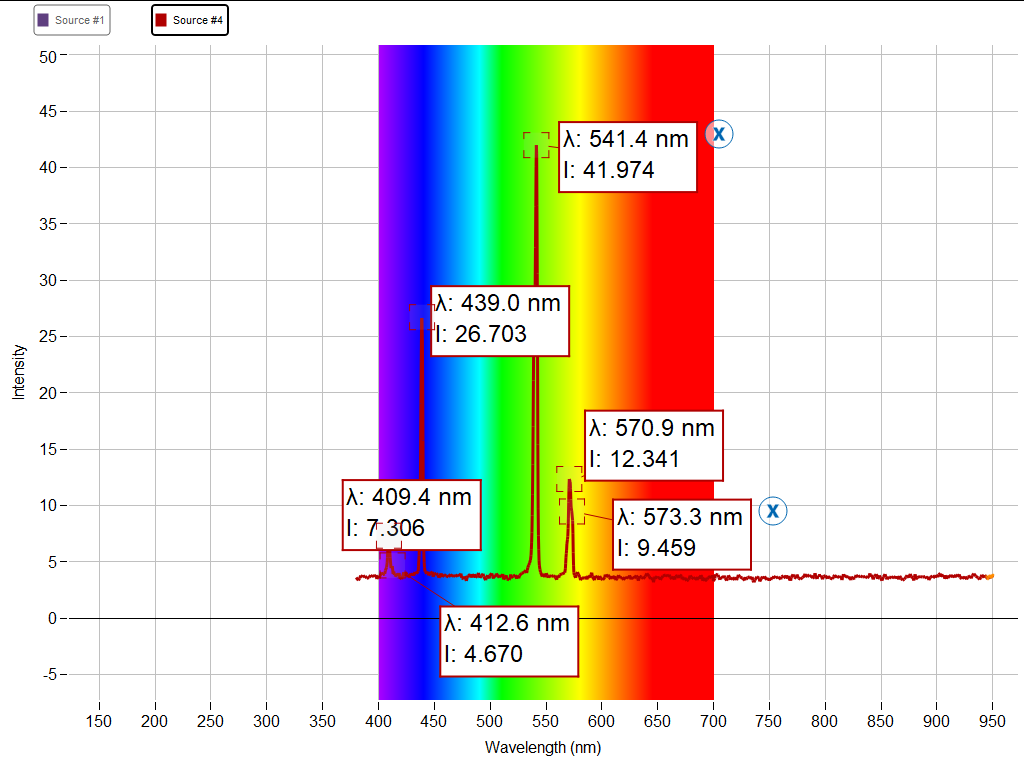
\includegraphics[width=0.8\textwidth]{Results/photospectrometry/mercury.png}
    \caption{Spectral Lines of Mercury}
    \label{fig:mercury_spectrum}
\end{figure}

\subsection{Part 2: Hydrogen Spectrum}
\begin{figure}[H]    \centering
    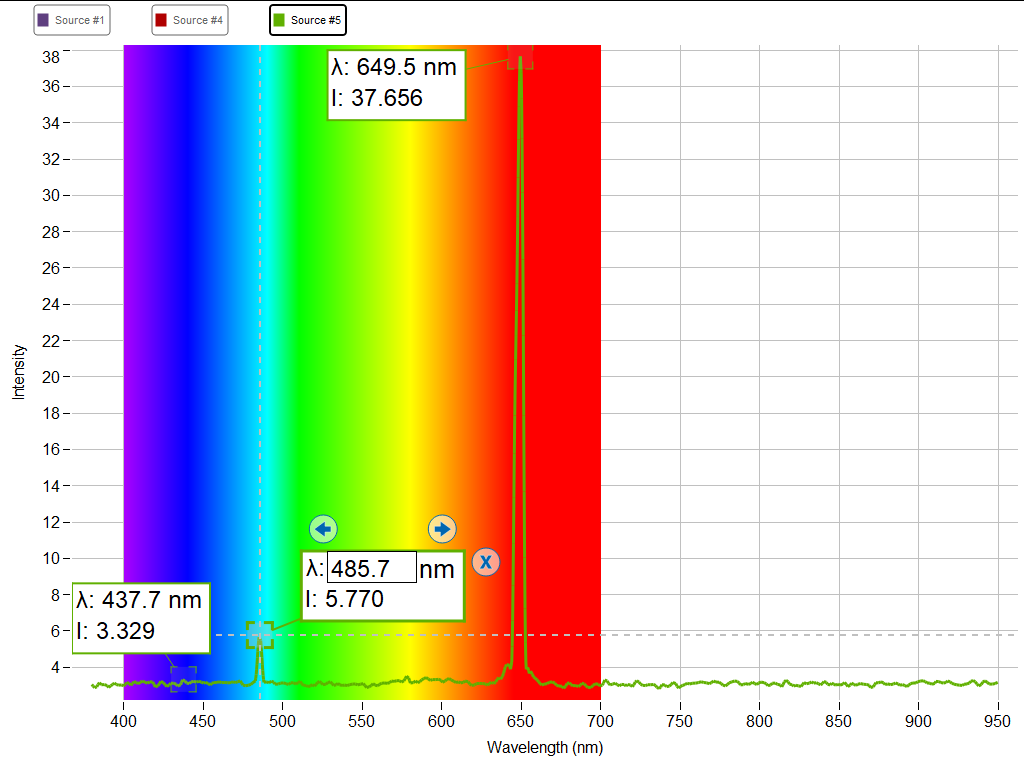
\includegraphics[width=0.8\textwidth]{Results/photospectrometry/hydrogen.png}
    \caption{Spectral Lines of Hydrogen}
    \label{fig:hydrogen_spectrum}
\end{figure}

\subsection{Part 3: Helium Spectrum}
\begin{figure}[H]    \centering
    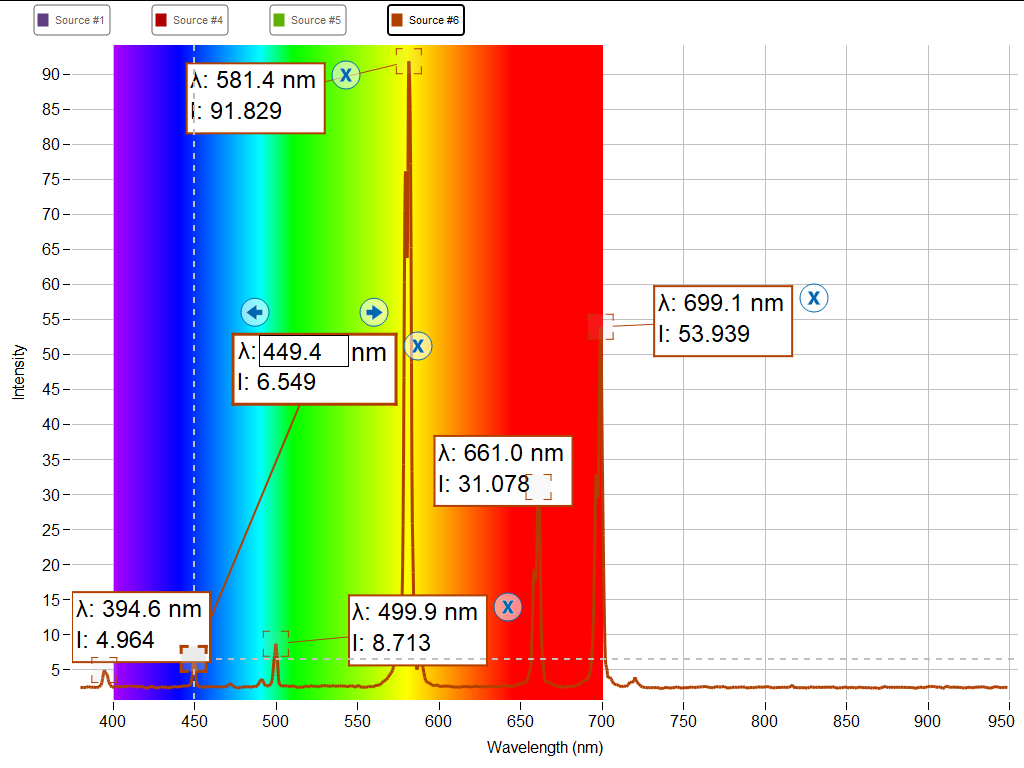
\includegraphics[width=0.8\textwidth]{Results/photospectrometry/helium.png}
    \caption{Spectral Lines of Helium}
    \label{fig:helium_spectrum}
\end{figure}

\subsection{Part 4: Unknown Spectrum}
\begin{figure}[H]    \centering
    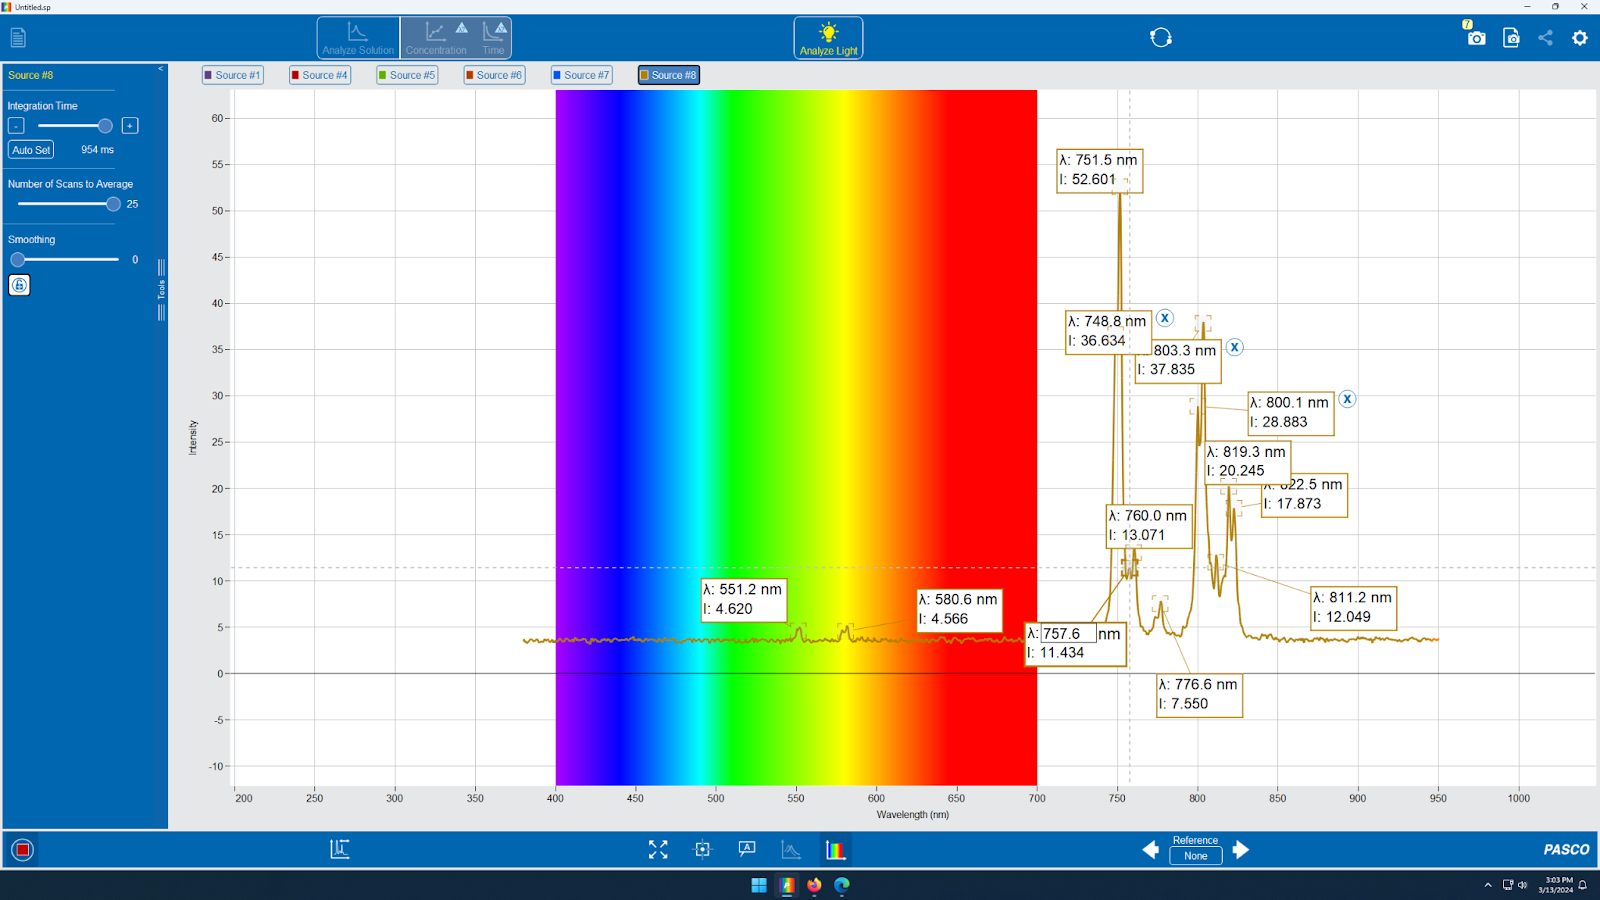
\includegraphics[width=0.8\textwidth]{Results/photospectrometry/unknown.png}
    \caption{Spectral Lines of Unknown Gas}
    \label{fig:unknown_spectrum}
\end{figure}

\subsection{Part 5: Absorbance of Dyes}
\begin{figure}[H]    \centering
    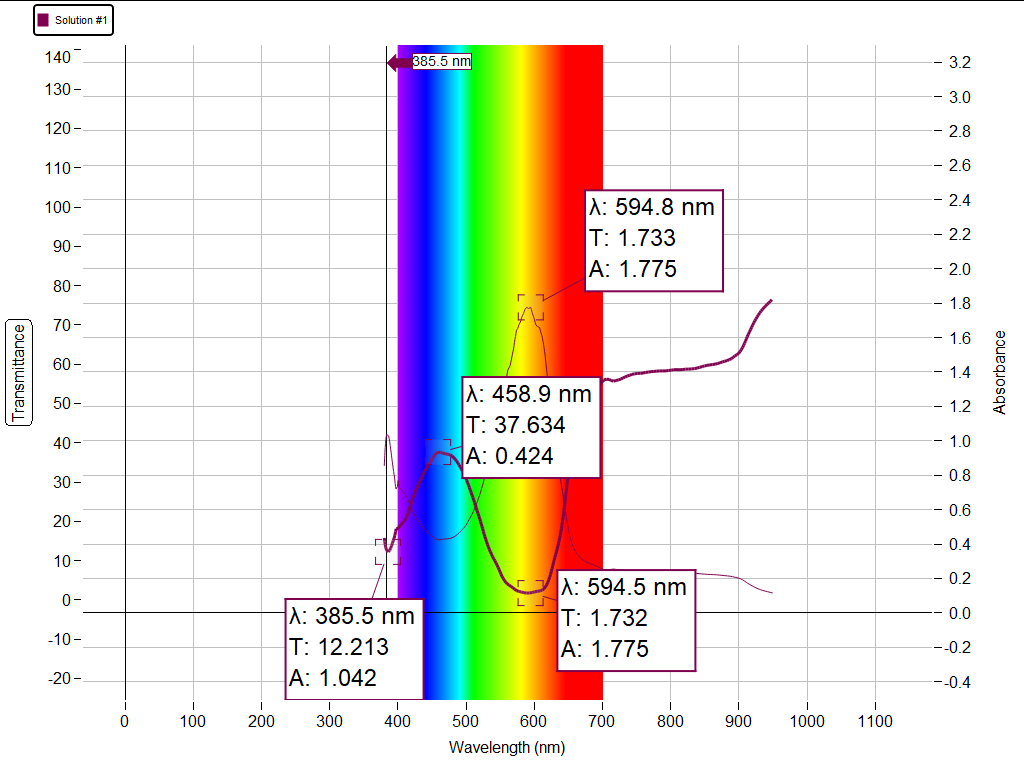
\includegraphics[width=0.8\textwidth]{Results/absorption_spectrometry/blue.png}
    \caption{Absorbance and transmittance of blue dye}
    \label{fig:blue_spectrum}
\end{figure}

\begin{figure}[H]    \centering
    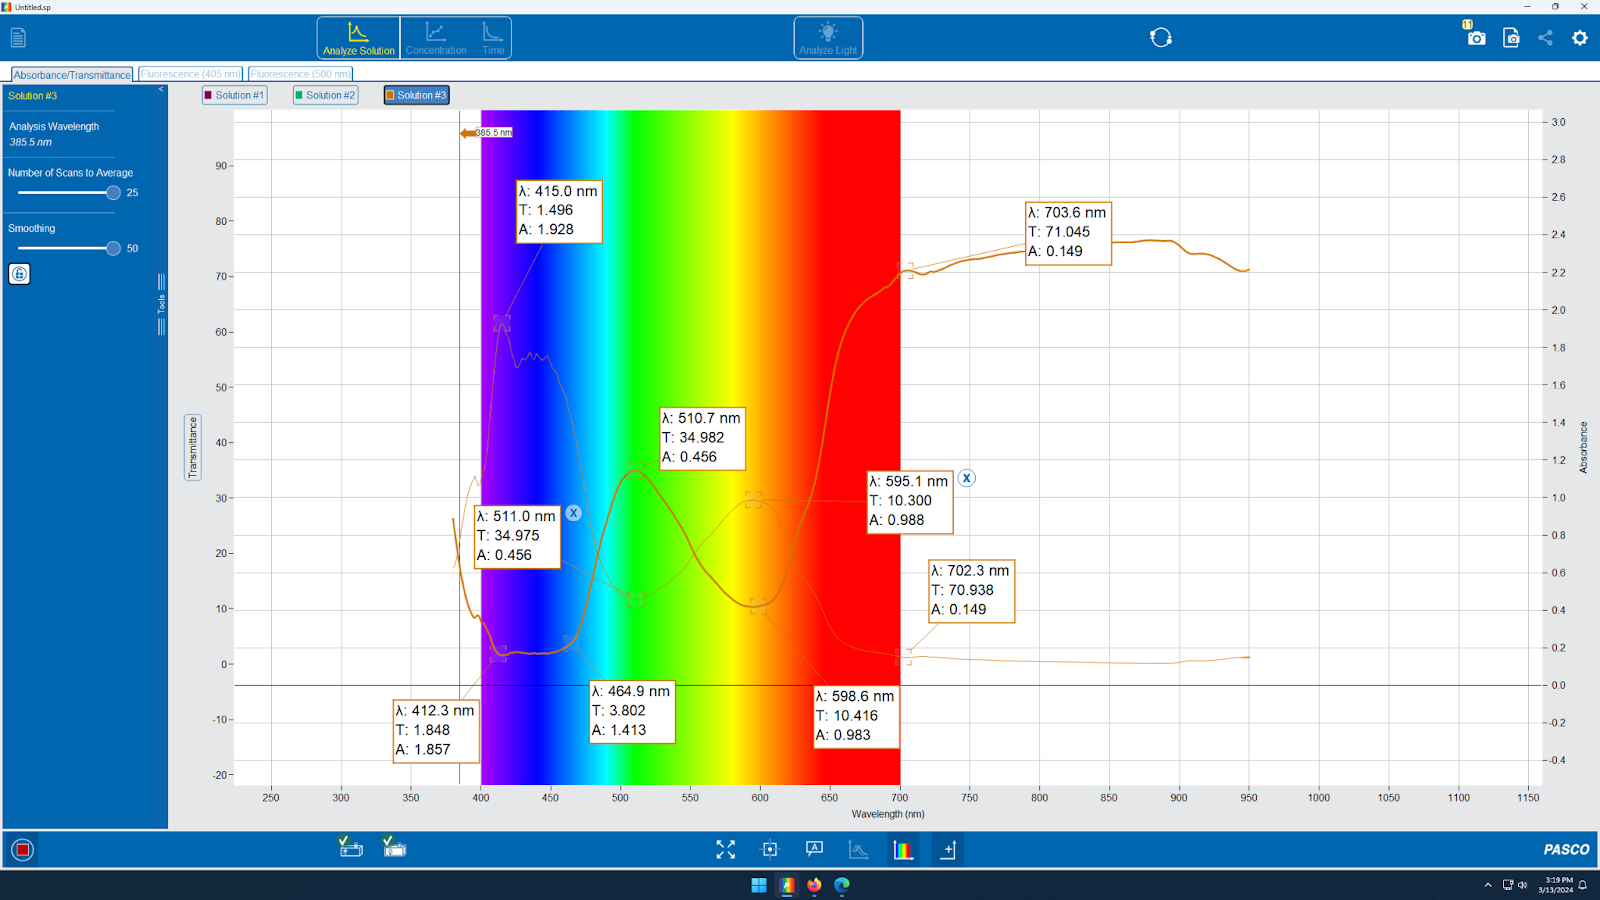
\includegraphics[width=0.8\textwidth]{Results/absorption_spectrometry/green.png}
    \caption{Absorbance and transmittance of green dye}
    \label{fig:green_spectrum}
\end{figure}

\subsection{Part 6: Fluorescence Spectrum}
\begin{figure}[H]    \centering
    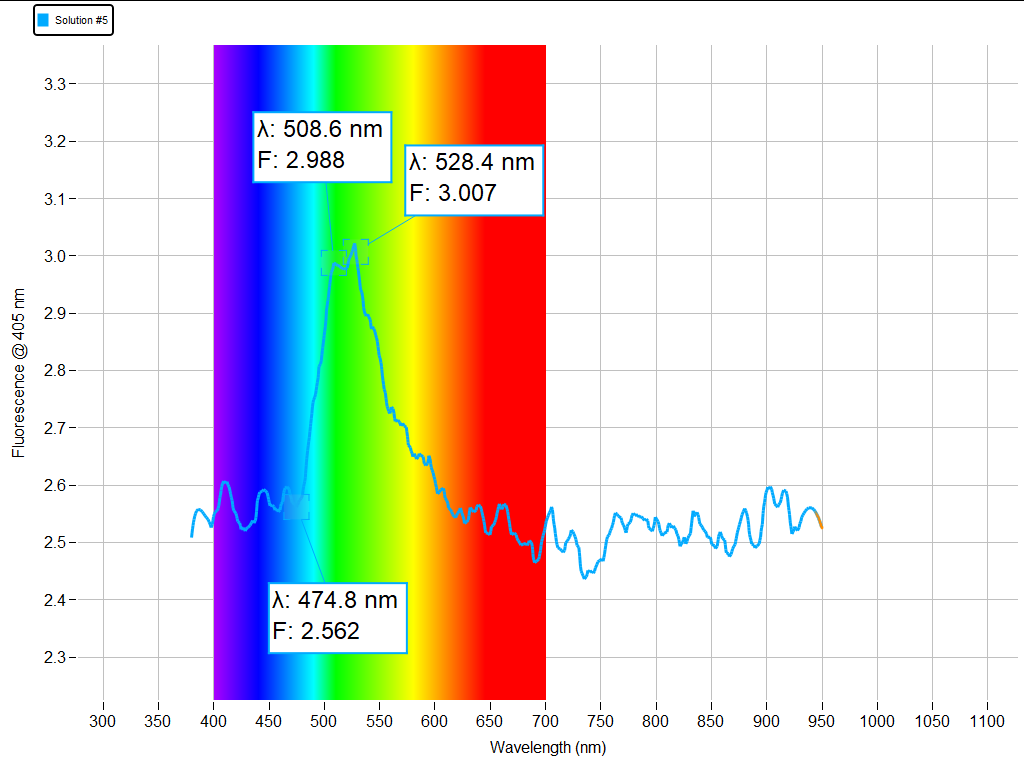
\includegraphics[width=0.8\textwidth]{Results/fluourescence_spectrometry/405nm.png}
    \caption{Fluorescence spectrum of yellow dye excited with 405nm light}
    \label{fig:fluorescence}
\end{figure}

\begin{figure}[H]    \centering
    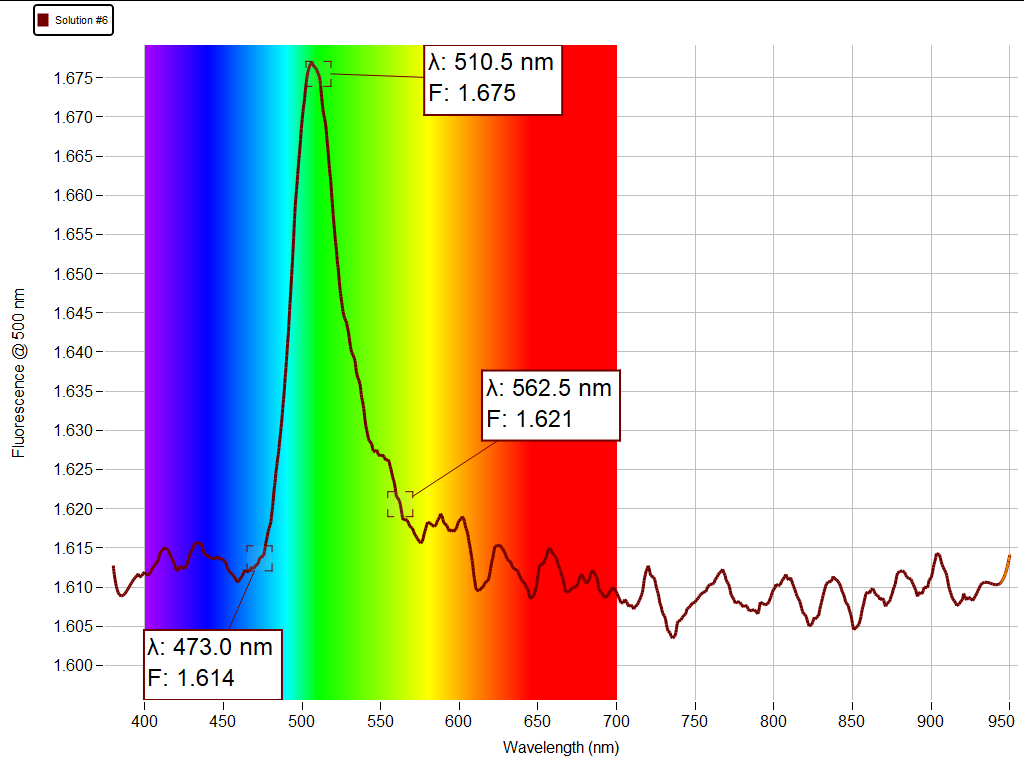
\includegraphics[width=0.8\textwidth]{Results/fluourescence_spectrometry/500nm.png}
    \caption{Fluorescence spectrum of yellow dye excited with 500nm light}
    \label{fig:fluorescence2}
\end{figure}